\documentclass{ECOS_2021}
%\usepackage{timesnew}
\usepackage{times}
\usepackage{graphicx}
\usepackage{amsmath}
\usepackage{amsfonts}
\usepackage{amssymb}
\usepackage{mathtools}
\usepackage{enumitem}
\usepackage{cite}
\usepackage{gensymb}
\makeatletter
\let\NAT@parse\undefined
\makeatother
\usepackage{hyperref}

%\renewcommand{\rmdefault}{phv} % Arial
%\renewcommand{\sfdefault}{phv} % Arial

\title{\sffamily ECOS 2021: Template for manuscripts  \\ - next line of the title}
\rmfamily
\author{First A. Author$^{a}$, Second B. Author$^{b}$, Third Author$^{c}$ and Fourth Author$^{d}$}

%\heading{First A. Author, Second B. Author and Third C. Author}

\address{$^{a}$ Institution,
City,
Country,
e-mail
\and
$^{b}$ Institution,
City,
Country,
e-mail
CA
\and
$^{c}$ Institution,
City,
Country,
e-mail
\and
$^{d}$ Institution,
City,
Country,
e-mail}

\abstract{\small Manuscript submitted to ECOS Conference must describe original, previously unpublished work (in a journal or a conference with refereed proceedings), and must not be simultaneously submitted or be under review for publication elsewhere. Authors are kindly requested to prepare the manuscript by using This template. Please note that detailed info on paper preparation can be found from Section 2.}

\keywords{\small Thermodynamics, Energy, ECOS Conference, Exergy, Sustainability.}

\begin{document}

% \thispagestyle{empty}

\sffamily \Large \section{Introduction} \label{Introduction} 
\rmfamily \normalsize 
Papers that already appeared in unpublished or informally published workshop proceedings may be submitted (in this case please cite the prior publication in the list of references and contact the ECOS International Scientific chair for permission). Information on Ethics in Publishing and Ethical guidelines for journal publication see at: \url{http://www.elsevier.com/publishingethics} and \url{http://www.elsevier.com/ethicalguidelines}.

\sffamily \large \subsection{Submission} \label{Submission}
\rmfamily \normalsize
Authors are requested to submit their manuscripts, using EasyChair platform by accessing the Conference page \url{http://ecos2020.org/} and, through the submission login, authors should upload the full manuscript file.

\sffamily \large \subsection{Information} \label{Information}
\rmfamily \normalsize 
Any doubts regarding the submission process should be sent to the organization committee contact, through the e-mail \href{mailto:ecos2020@amano.mech.waseda.ac.jp}{ecos2020@amano.mech.waseda.ac.jp}.

\sffamily \Large \section{General information about ECOS 2020 papers} \label{General}
\rmfamily \normalsize 
\sffamily \large \subsection{Manuscript preparation process} \label{Manuscript preparation process}
\rmfamily \normalsize 
The manuscript must be prepared in English (British or American spelling) and free of grammatical, spelling and/or punctuation errors. The manuscript must be thoroughly edited and proof-read before it is submitted. Authors have the responsibility to ensure clear and adequate English expression, since indecipherable language could be a valid reason for rejection of the paper.
Units in the paper must be according to the International System of Units (SI, Systme International d'Units). Other units may be given in parentheses (when they first appear in the text), dual-unit tables, or an appendix.

Authors are kindly requested to prepare the manuscript by using this template. {\bf The manuscript length is limited to twelve (12) pages at the maximum.}

The template documents contain necessary information regarding desktop publishing format, type sizes, and typefaces. Formatting styles are classified in four groups:

\sffamily \large \subsection{Manuscript submission and review process} \label{Manuscript submission and review process}
\rmfamily \normalsize 
Authors are requested to submit their manuscript, with page numbers, as Portable Document Format (PDF) file for the review process and as the \LaTeX{} file package for the ECOS Conference proceedings.

For each submission that falls within the scope of the ECOS Conference, independent experts in the field of the submission will be selected to act as reviewers. ECOS Conferences use a single-blind peer review process where the identity of the reviewers will remain anonymous\footnote{The identity of the authors will be known to the reviewers.}. The appropriate editor will assess the recommendation report from the reviewers as to whether the article should be accepted, revised or rejected. The submitted manuscript, subject to final acceptance on the basis of the reviewers report, will be included in the conference proceedings without any modifications.

\sffamily \Large \section{Organization of paper} \label{Organization of paper}
\rmfamily \normalsize
The basic parts of a paper are listed below in the order in which they should appear:

\begin{itemize}
    \item Title (Section \ref{Title}).
    \item Author(s), author's (or authors') affiliation(s), Corresponding author identifier (Section \ref{Authors information}).
    \item Abstract and Keywords (Section \ref{Abstract and keywords}).
    \item Subject matter of the paper with numbered main headings and sub-headings (Section \ref{Subject}).
    \item Acknowledgments, if any, (Section Acknowledgments).
    \item Appendices, if any, (Section Appendix A, Appendix B).
    \item Nomenclature with SI units, if any, (Section Nomenclature).
    \item References (Section References).
\end{itemize}

\sffamily \large \subsection{Title} \label{Title}
\rmfamily \normalsize
The article title appears centred at the top of the first page. To format the title authors should use the “Title” style from the formatting menu. Only the first word and proper nouns for the title should be capitalized.The  use  of  acronyms  and  abbreviations  in  the  title  should  be  avoided,  unless  they  are widely understood, or they are accompanied by the expanded expression.

\sffamily \large \subsection{Authors information} \label{Authors information}
\rmfamily \normalsize
The author's name should include first name, middle initial and
surname (e.g. Nikola Tesla, not Tesla Nikola, Ben Roethlisberger, not Roethlisberger Ben; Ming Yao, not Yao Ming). It should be written centered, in 12pt boldface Roman,
12pt below the title.

Author's affiliation should be written centered, in 11pt Roman, 12pt below the list of authors. A 2pt space should separate two different affiliations. Each affiliation must include, at the very least, the name of the institution, country and e-mail addresses. For multiple affiliations, each affiliation should appear in a separate line. Author names and affiliations are linked with superscripts. Corresponding author identifier (CA) should be put after the affiliation of corresponding author. This information is compulsory for the submission process.

\sffamily \large \subsection{Abstract and keywords} \label{Abstract and keywords}
\rmfamily \normalsize
The abstract and keywords follow the title and author information. Please, try to write five key words. They should be written left aligned, in 12pt Roman, and the line must begin with the words {\bf Key words}: boldfaced. The first letter of each keyword or keyword phrase should be capitalized; the keywords or phrases should be separated from one another by commas, with a period (full stop) following the last one. A 12pt space should separate the key words from the affiliations.

Abstract section should consist of a single paragraph containing no more than 300 words, and should be formatted in 12pt Roman. Abbreviations and acronyms should be expanded when they appear for the first time in the abstract.

\sffamily \large \subsection{Subject matter of the paper with numbered main headings and sub-headings} \label{Subject}
\rmfamily \normalsize
The subject matter (body) of the paper should be composed of main sections, each preceded by a main heading - the main headings should be written left aligned, in 12pt, boldface Roman letters. The sub-sections should be preceded by the secondary headings should be written left aligned, 12 pt, boldface Roman, with an initial capital for first word only. There should be a 12pt space before and 6pt after the both main and secondary headings.

Main headings of sections Nomenclature, References, Acknowledgments and Appendix are unnumbered.

Paragraphs that follow the headings should not be indented. The normal text should be written single-spaced, justified, using 12pt (Times New) Roman in one column. There is not an inter-paragraph spacing. During the text preparation authors may:

Manually format any special text that need to be italicized, bolded, subscripts or superscripts. For emphasis the boldface should be used, while underlining is not recommended in manuscript. The use of different fonts (usually symbol font) for special purpose should be avoided; instead authors should use the symbols.

Abbreviations and acronyms should be expanded when they appear for the first time in the text, even if they have already been defined in the title or abstract. Abbreviations that incorporate periods should not have spaces: write ``C.N.R.S.,'' not ``C. N. R. S.'' Chemical compounds should be named according to the systematic rules of the IUPAC or Chemical Abstracts.

Footnotes should be kept to a minimum and used only for substantive observations. Endnotes should not be used at all.

\sffamily \subsubsection{Displayed list: Bulleted list and number list} \label{List}
\rmfamily
Displayed list is a list that is set off from the text, as opposed to a run-in list that is incorporated into the text. There is no strict rule when to create the display list, but within the text lists should not have more than three items. For example, within the text lists would appear: 1) using a number, 2) followed by a close parenthesis.

The bulleted list should be defined with \textit{itemize} environment like below :
%
\begin{itemize}
    \item Use a colon to introduce the list.
    \item Template uses predefined bullets instead of checks, arrows, etc. for bulleted lists.
    \item Tab spacing within the lists is also predefined.
\end{itemize}
%
The numbered list with \textit{enumerate} environment:
%
\begin{enumerate}
    \item Use a colon to introduce the list.
    \item Labels should not be numbers enclosed in parentheses because such labels cannot be distinguished from equation numbers.
    \item Tab space between symbol and text is 0.5 cm.
\end{enumerate}
%
If more depth within the list is needed, lists can be nested.
%
\begin{itemize}
    \item Top level
    \begin{itemize}
        \item Second level
    \end{itemize}
\end{itemize}

\sffamily \subsubsection{Equations and expressions} \label{Equations and expressions}
\rmfamily
Equations should be centered in a separate line with spacing before and after, with use of \textit{equation} environment. Applying the proposed environment ensures that equations will be numbered automatically with Arabic numbers in parentheses.
%
\begin{equation}
        y=a_{j}x_{j}+\left( a_{j}b_{j}+\epsilon_j\right)
        \label{EQN1}
\end{equation}
%
A recommended order of closures for parenthesis, brackets and braces, is the following:
%
\begin{equation}
        \left\{ \left[ \left(\dotsc \right) \right] \right\}
        \label{EQN2}
\end{equation}
%
Authors should refer to equations in the text by (\ref{EQN1}), not by ``Eq. (\ref{EQN1})" or ``Equation (\ref{EQN1})" except at the beginning of a sentence: ``Equation (\ref{EQN1}) is used...". If there are chemical formulae included, i.e. reactions, please number them (R1), (R2), etc. Complicated chemical structures should ideally be prepared with chemistry drawing software (e.g. ChemDraw, Chem Windows, ISIS/Draw) and treated like figures.

Expressions which are simple, short, and not of major importance can be left in the text, and written in one-line form (e.g., use $\beta = a/b$ for fractions). ). For expressions within a line of text authors should use regular text and the symbols like:
\begin{itemize}
    \item For binary operations:
    \begin{itemize}
        \item Plus sign $(+)$.
        \item Minus sign $(-)$.
        \item Multiplication sign $(\dot)$ or $(\times)$.
        \item Fractional sign slash $/$ or division sign $(\div)$.
        \item Composition sign $(\degree)$, also degree sign.
    \end{itemize}
    \item For binary relations $=,\neq,<,>$ and $|$.
\end{itemize}

Symbols in equations and expressions must be defined in the Nomenclature, or in some cases immediately following them.

\sffamily \subsubsection{Figures and Tables} \label{Figures and Tables}
\rmfamily
Figures and tables are most effective when they are clear, self-explanatory, accurate, easily understood and remembered. In general, tables and figures should have enough explanation in their captions to stand alone.

Tables and figures (graphs, charts, drawing, and photographs) must be embedded in the document. They should be placed between paragraphs, after (or near) their first mention in the text. Note that the arrangement of the elements may slightly change after applying all the text formatting.

Figure captions have to be placed below the figures and table titles have to be placed above the tables. Authors should include a minimum of one sentence summarizing what the figure/table shows or illustrates in the text; also verify that the figures and tables mentioned in the text actually exist.

All of tables and figures should be numbered consecutively and captioned; the caption should be 10pt Roman, upper and lower case letters.

\sffamily \subsubsection{Figures} \label{Figures}
\rmfamily
The recommended font in artwork is Times New Roman, same size as the text. Figure lettering should be large enough to be legible when the size of the drawing is reduced. Axes titles on graphs must be labelled with words rather than symbols. As an example, vertical axe in Fig. 1 is labelled as the quantity ``Pressure" or ``Pressure, {\it p}1" not just ``{\it p}" or ``{\it p}1". Units should be put in parentheses.

If a figure has two (or more) parts, authors should include labels ``(a)",``(b)" as part of the artwork. Figures are going to be reproduced in colour in the electronic versions of the Proceedings, but in the journals they will be printed in black and white. Therefore, distinctions have to be used so that images can still be understandable in black and white printings.

For easier manuscript preparation authors are advised to create separate figure files and convert them into proper file format. For ECOS proceedings TIF (raster artwork) and EPS (vector artwork) are the preferred formats; JPG, GIF formats are acceptable. It is important to understand that the non-preferred formats are not ideally suited to high-quality image reproduction, and are not acceptable for conversion to a paper that may be considered for archival journal publication.

\begin{figure}[h!]

    \centering
    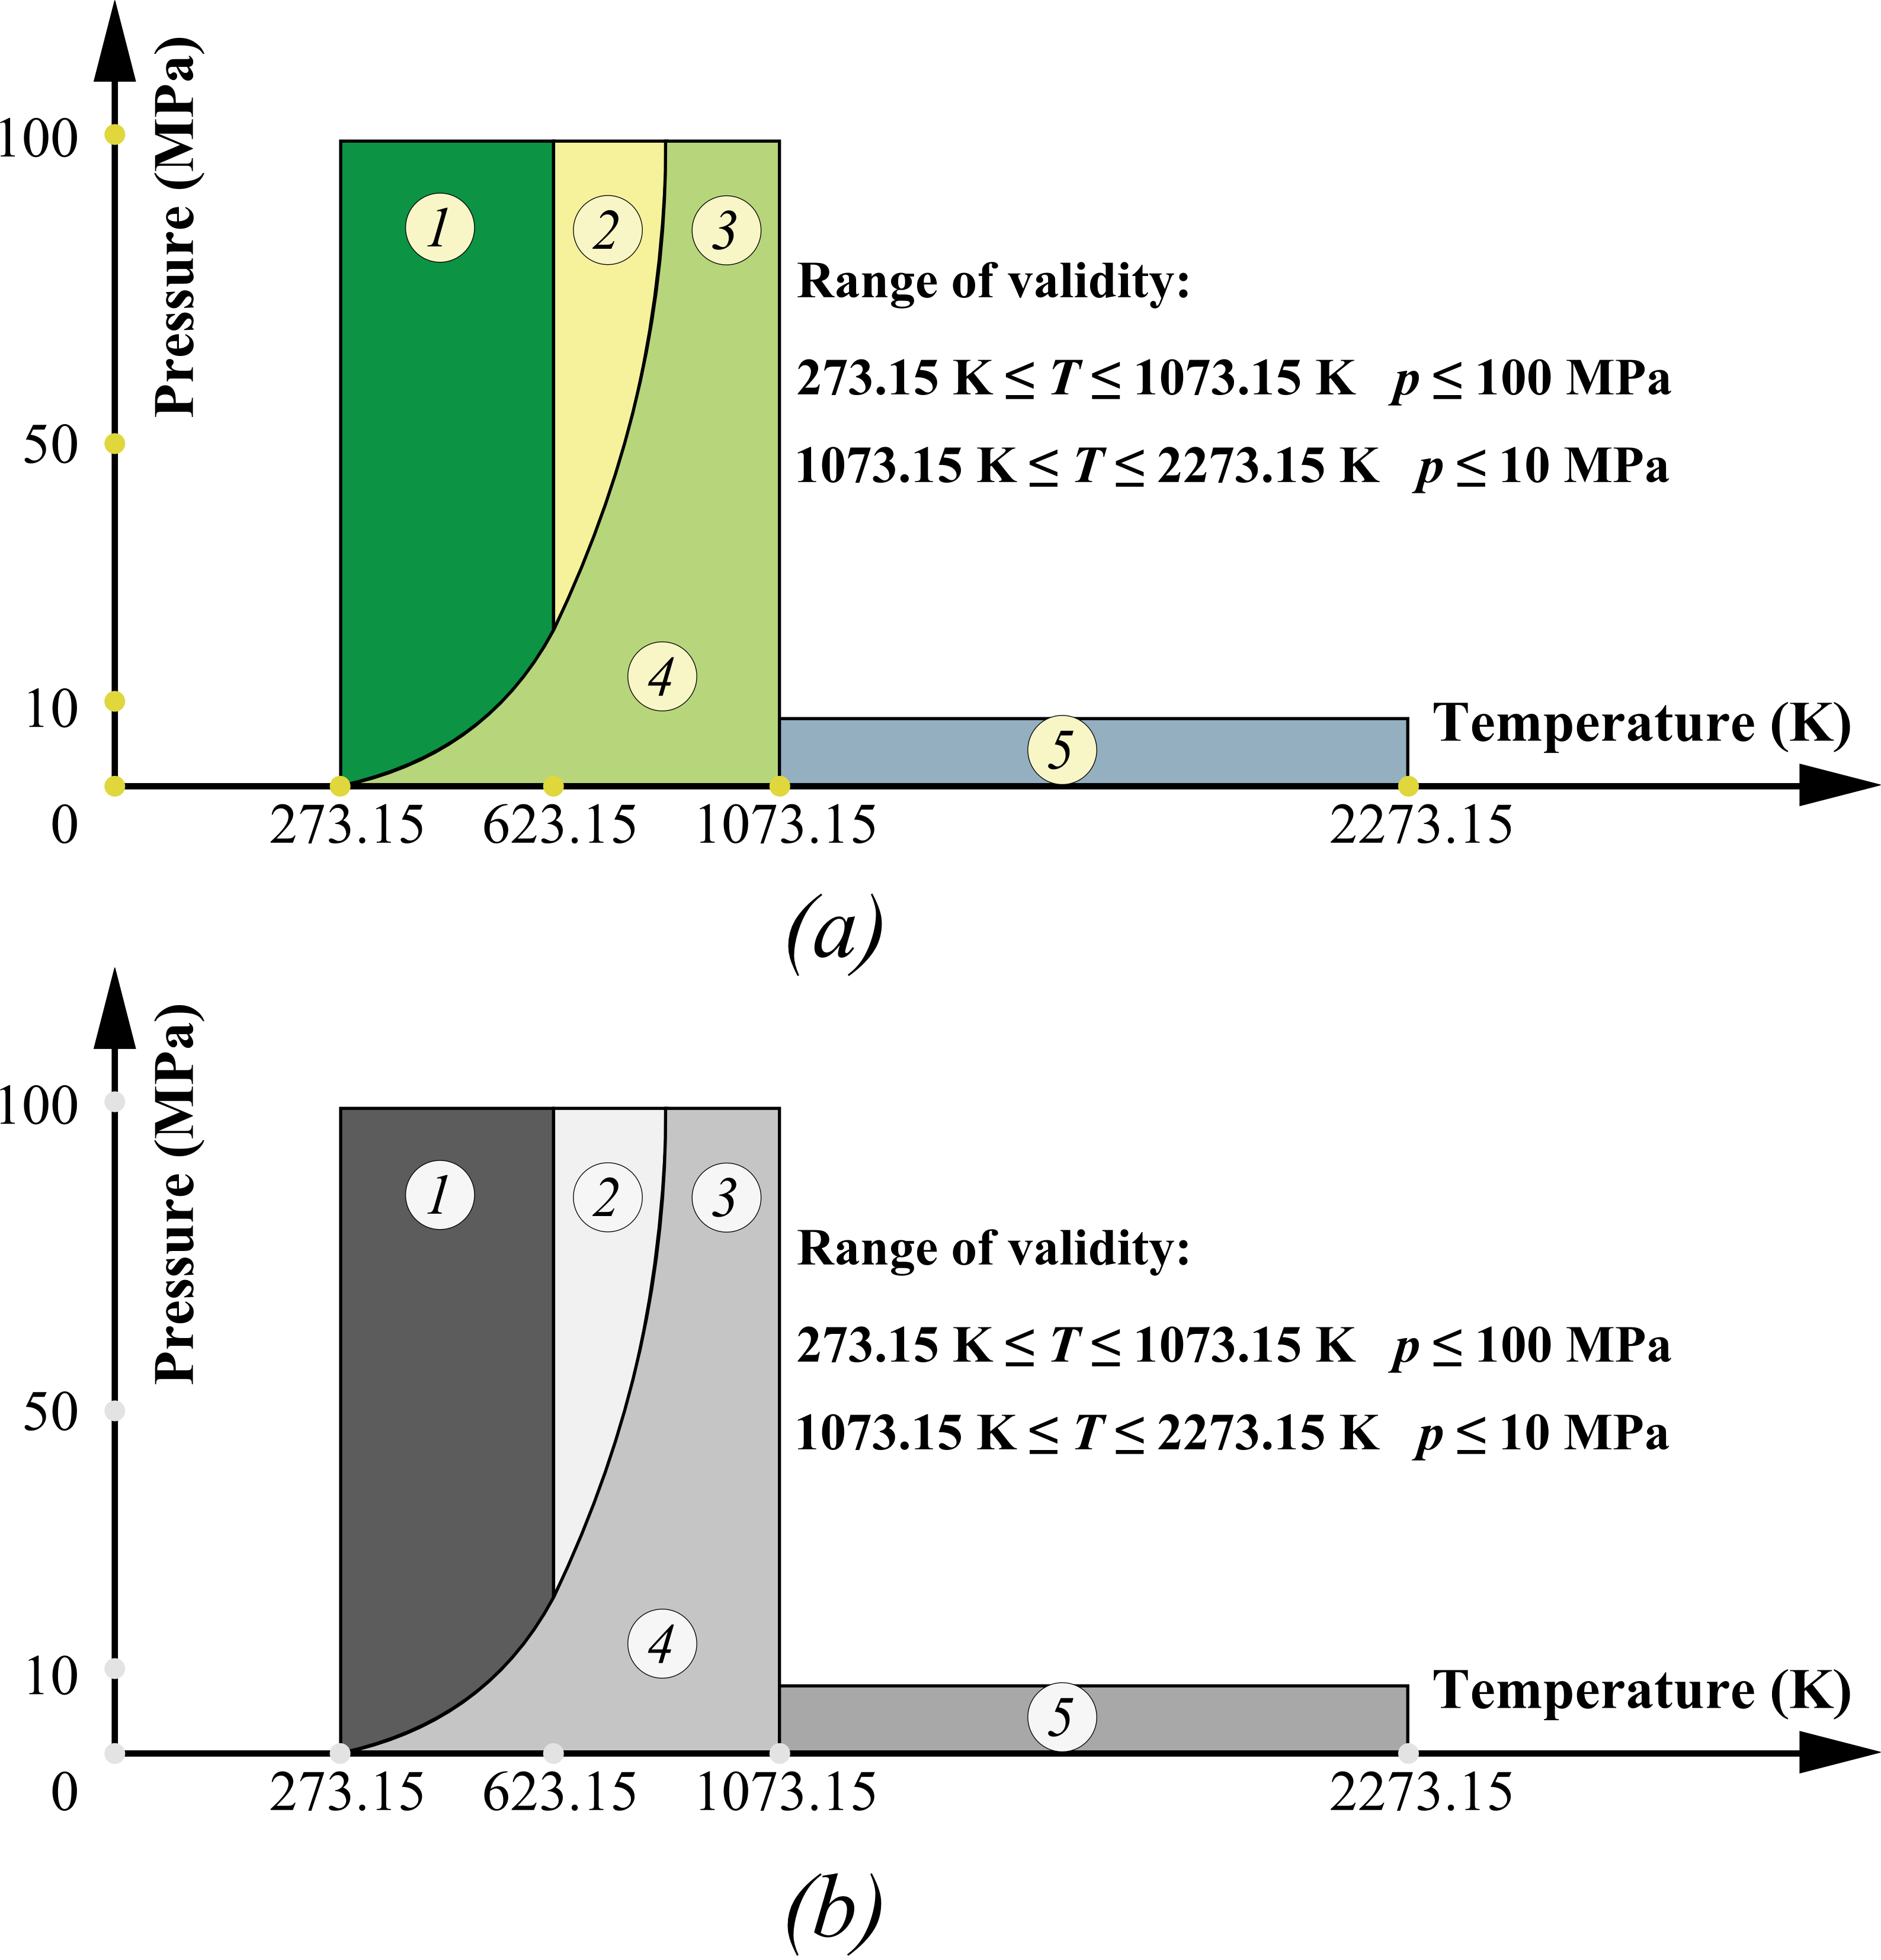
\includegraphics{Figure_1.png}
    \caption{Use of appropriate contrasted colours for black and white printing: a) colour figure, b) greyscale figure.}
    \label{Fig_1}       % Give a unique label
\end{figure}

Before inserting in the document each figure should be:

\begin{itemize}
    \item Prepared as simply as possible for clarity. Avoid sideways illustrations if possible.
    \item Sized to the desired final dimensions in order to minimize the final document file size.
    \item Prepared with at least 300 dpi resolutions for raster artwork (greyscale and colour halftones), 600 dpi for combinations (line art and halftone together) and 1200 dpi for line art.
\end{itemize}

To embed (insert) images, prepared in separate files, authors should use \textit{figure} environment. If the authors are providing scanned figures, they have to be clear, with all the legends and data labels easily readable. If this is not possible, the author must redraw the figures especially in the case of simple ones. Illustrations borrowed or adapted from another source have to be properly acknowledged. Figure caption should be below the figure.

When a figure is referred to in the text, it should be typed as Fig \ref{Fig_1} or Figs 2 to 4, with ``Fig." capitalized and abbreviated (unless it is the first word in a sentence) and without period at the end (unless the reference appears at the end of a sentence).

\sffamily \subsubsection{Tables} \label{Tables}
\rmfamily
All tables should be prepared using \textit{table} environment. Tables should be numbered consecutively and captioned, the caption should be 10pt Roman, upper and lower case letters. Table caption should be above the Table.

Tables should be as simple as possible, with single horizontal lines above and below column headings and subheadings, and at the bottom of the table (if it is necessary the authors may put horizontal lines between the rows). Limit the number of columns to fewer than 10, since the use of many columns will create readability problems. Vertical lines and shaded areas should be avoided where possible. Fancy frames or borders around tables should not be used.

\begin{table}[h]
\caption{Table format in ECOS: Template for manuscripts}
\begin{center}
\begin{tabular}{*{4}{c}}
\hline
Month & $\rho_{cs}$, \% & $\rho_{ps}$, \% & $\rho_{os}$, \%\\
\hline
JAN & 5.88 & 36.88 & 57.24 \\
FEB & 6.79 & 45.65 & 47.57 \\
MAR & 5.48 & 40.40 & 54.12 \\
APR & 16.39 & 51.58 & 32.03 \\
MAY & 11.18 & 45.27 & 43.55 \\
JUN & 12.87 & 33.68 & 53.45 \\
JUL & 15.94 & 40.45 & 43.62 \\
AUG & 6.10 & 50.22 & 43.68 \\
\hline
\end{tabular}
\end{center}
\label{Table_1}
\end{table}

When Tables are referred to in the text, they should be typed as Table \ref{Table_1} or Tables 2 to 4. Authors should not abbreviate ``Table" and should not put period after number, unless the reference appears at the end of a sentence.

\sffamily \Large \section*{Acknowledgments}
\rmfamily \normalsize
Any acknowledgments authors wish to make should be included in a separate section with normal formatting, at the end of the main text and before the appendix (if any), nomenclature and references section. This section starts with headings Acknowledgments.

\sffamily \Large \section*{Appendix}
\rmfamily \normalsize
An Appendix, if needed, should appear after the acknowledgments.

\sffamily \Large \section*{ Nomenclature}
\rmfamily \normalsize
If symbols are used extensively, paper must have a separate Nomenclature section. Section starts with a heading Nomenclature. This section lists in detail all the symbols used in the text and their definitions. The list should include:
%
\begin{itemize}
    \item Letter symbol; each symbol used in a paper should have a unique definition.
    \item Accurate and concise definition of symbol. Definitions do not require ''the'' and are followed by comma and one space.
    \item Units of measure used in the paper. No end punctuation in nomenclature.
\end{itemize}
%
All Letter symbols (dimensional and dimensionless) should be listed in an alphabetic order. Letter symbols are followed by Greek symbols, subscripts and superscripts.

%\begin{nomenclature}
%    \item[$\dot m_k$]   stream of $k$-th harmful substance leaving balance boundary of power unit,
%    \item[$N_{el}$] net electric power but not with concentration,
%    \item[$P_{k,el}$] amount of $k$-th harmful substance burdening the production of electricity.
%\end{nomenclature}
\vspace{6pt}
\textbf{Example}
\begin{description}[leftmargin=!,labelwidth=\widthof{maxlength}]
    \item[$c$] specific heat, ${\rm J/(kgK)}$
    \item[$h$] heat transfer coefficient, ${\rm W/m^{2}K}$
    \item[$\Dot{m}$] mass flow rate, ${\rm kg/s}$
    \item[$t$] temperature, ${\rm ^\circ C}$
\end{description}

\textbf{Greek symbols}
\begin{description}[leftmargin=!,labelwidth=\widthof{maxlength}]
    \item[$\eta$] efficiency
    \item[$\phi$] maintenance factor
\end{description}

\textbf{Subscripts and superscripts}
\begin{description}[leftmargin=!,labelwidth=\widthof{maxlength}]
    \item[a] Air
\end{description}

\sffamily \large \subsection{Citations}
\rmfamily \normalsize
Authors should acknowledge the reference sources (either from a printed document or from the web) whenever they:
%
\begin{itemize}
    \item Paraphrase or summarize another person's ideas or points.
    \item Quote another person's work.
    \item Use information from any source, including information contained in tables, graphs, figures or diagrams.
\end{itemize}
%
ECOS uses the numeric system of referencing, according to the conventions set down in the Vancouver/Numeric style. References to cited literature should be numbered consecutively throughout the paper and collected together in a section References.
In the text, each reference number (Arabic numerals) should be enclosed in square brackets in the same line as the text (\cite{journal}, \cite{proceedings}), before any punctuation such as: full stops, commas, colons and semi-colons. Author should refer to the reference number, and do not use ``Ref. \cite{chapter}" or ``reference \cite{chapter}" except at the beginning of a sentence: ``Reference \cite{chapter} was..." When multiple references are cited at a given place in the text, author should:
%
\begin{enumerate}
    \item Use a hyphen to join the first and last numbers that are inclusive: \cite{proceedings,chapter,books,report}.
    \item Use commas (without space) to separate no inclusive numbers in a multiple citation \cite{proceedings,chapter,books,report, web_references}.
\end{enumerate}
%
A reference to a particular article or chapter in a book may be cited in the text multiple times but must only appear once in the reference list. During the text preparation authors are encouraged to:
\begin{itemize}
    \item Substitute reference numbers for the name of the author whenever appropriate:
    \begin{itemize}
        \item As Smith, Wesson and Ruger, and Williams et al. demonstrate, {\bf incorrect}.
        \item As \cite{journal}, \cite{proceedings}, and \cite{chapter} demonstrate, {\bf correct}.
        \item As Smith \cite{journal}, Wesson and Ruger \cite{proceedings}, Williams et al. (for more than 2 co-authors) \cite{chapter}.{\bf correct}.
    \end{itemize}
    \item Place numbers directly after the reference rather than at the end of a clause or sentence, (unless the reference ends at the end of a clause or sentence).
    \begin{itemize}
        \item One study examined the energy efficiency in ... \cite{journal}, {\bf incorrect}.
        \item One study \cite{journal} examined the energy efficiency in ...., {\bf correct}.
    \end{itemize}
\end{itemize}

Authors must provide a full description of each source which has been cited in the text in a references list. The information must be sufficient to make it possible for interested readers to easily locate and obtain the source. The references should be listed in the same order as cited in the text, not in alphabetical order.

References to electronic data available only from personal Web sites or commercial, academic, or government ones where there is no commitment to archiving the data, should be avoided. Depending on the circumstances, private communications, Web site addresses, citations like ``In preparation" and ``To be submitted" may be incorporated into the main text of a paper or may appear in appendix. The following examples demonstrate the format for a variety of types of references.

Citations should be given according to the examples in the section References for articles in journals \footnote{Journal titles can be abbreviated, see URL: http://www.efm.leeds.ac.uk/~mark/ISIabbr/.} \cite{journal}, \cite{journal2} and proceedings \cite{proceedings}, chapter in book \cite{chapter} as well as for books \cite{books}, technical reports \cite{report}, dissertations \cite{dissertation} and web available sources \cite{web_references}.

\sffamily \Large
\begin{thebibliography}{99}
\rmfamily \normalsize

\bibitem{journal} Sciacovelli A., Verda V.
\textit{Entropy generation analysis in a monolithic-type solid oxide fuel cell (SOFC)}. Energy 2009;34(7):850-65.

\bibitem{journal2} Yapici H., Kayatas N., Albayrak B., Basturk G.,
\textit{Numerical calculation of local entropy generation in a methane air burner}. Energy Convers Manage 2005;46:1885-919 \footnote{If a journal carries continuous pagination throughout a volume the month and issue number may be omitted.}.

\bibitem{proceedings} Bolliger R., Favrat D., Maréchal F.,
\textit{Advanced Power Plant Design Methodology using Process Integration and Multi-Objective Thermo-Economic Optimisation}. In: Kjelstrup S., Hustad E., Gundersen T., Røsjorde A., Tsatsaronis G., editors. ECOS 2005: Proceedings of the 18th International Conference on Efficiency, Cost, Optimization, Simulation, and Environmental Impact of Energy Systems; 2005 Jun 20-25; Trondheim, Norway. Tapir Academic Press:777-84.

\bibitem{chapter}  El-Halwagy MM.
\textit{Sustainable pollution prevention through mass integration.}. In: Sikdar S, Diwekar U, editors. Tools and methods for pollution prevention. Dordrecht, Netherlands: Kluwer Academic Publisher. 1999. p. 233-76.

\bibitem{books}  Bejan A.
\textit{Shape and structure, from engineering to nature.}. Cambridge, UK: Cambridge University Press; 2000.

\bibitem{report}  Holland A., O’Sullivan B.
\textit{Weighted super solutions for constraint programs.} Cork, Ireland: University College Cork, Cork Constraint Computation Centre; 2004 Dec. Technical Report No.: UCC-CS-2004-12-02.

\bibitem{dissertation}  Magistri L.
\textit{Hybrid Systems for Distributed Generation [dissertation]} Genova, Italy: Università  di Genova; 2003.

\bibitem{web_references}  National Institute of Standards and Technology.
\textit{NIST-JANAF Thermochemical Tables} Available at: \url{http://kinetics.nist.gov/ janaf/} [accessed 12.3.2008].
\end{thebibliography}

\end{document}
